\documentclass[presentation, 10pt]{beamer}

\usepackage{booktabs}
\usepackage{tikz}
\usetikzlibrary{positioning}
\usepackage{booktabs}
\usepackage{amsmath}
\usepackage{pifont}
\newcommand{\cmark}{\ding{51}}
\newcommand{\xmark}{\ding{55}}
\DeclareMathOperator{\grad}{grad}
\DeclareMathOperator{\tr}{tr}
\let\div\relax
\DeclareMathOperator{\div}{div}
\DeclareMathOperator{\curl}{curl}
\date{November 23, 2018}
\usetheme{metropolis}
\metroset{progressbar=frametitle}

\usepackage{algpseudocode}
\renewcommand{\vec}[1]{\ensuremath{\boldsymbol{#1}}}
\newcommand{\ddt}[1]{\frac{\partial #1}{\partial t}}
\newcommand{\zhat}{\hat{\vec{z}}}
\newcommand{\W}{\ensuremath{\mathbb{W}}}

\newcommand{\inner}[1]{\left\langle #1 \right \rangle}

\newcommand{\KSP}[2]{\ensuremath{\mathcal{K}\left(#1, \mathbb{#2}\right)}}
\newcommand{\ksp}[1]{\KSP{#1}{#1}}

\newcommand{\highlight}[1]{\colorbox{red!20}{\color{black} #1}}
\newcommand{\arxivlink}[2]{%
  \href{http://www.arxiv.org/abs/#1}%
  {\texttt{arXiv:\,#1\,[#2]}}%
}
\newcommand{\doilink}[1]{%
  \href{http://dx.doi.org/#1}%
  {\texttt{doi:\,#1}{}}%
}

\author{Lawrence Mitchell\inst{1,*} \\ {\scriptsize C.J.~Cotter,
    P.E.~Farrell, D.A.~Ham, M.~Homolya, P.H.J.~Kelly, R.C.~Kirby, F.~Wechsung, \ldots}}
\institute{
  E333 (Christopherson)  

  \inst{1}Department of Computer Science, Durham University

  \inst{*}\texttt{lawrence.mitchell@durham.ac.uk}
}

\graphicspath{{./\jobname.figures/}{../pictures/}}

\usepackage[url=false,
doi=true,
isbn=false,
style=authoryear,
maxnames=5,
giveninits=true,
uniquename=init,
backend=biber]{biblatex}

\usepackage{xspace}
\let\Re\relax
\DeclareMathOperator{\Re}{Re}
\newcommand{\honev}{\ensuremath{{H}^1(\Omega; \mathbb{R}^d)}\xspace}
\newcommand{\ltwov}{\ensuremath{{L}^2(\Omega; \mathbb{R}^d)}\xspace}
\newcommand{\ltwo}{\ensuremath{{L}^2(\Omega)}\xspace}
\newcommand{\laplace}{\ensuremath{\Delta}\,}
\newcommand{\rt}{\ensuremath{\mathrm{RT}_0}\xspace}
\newcommand{\nd}{\ensuremath{\mathrm{ND}_0}\xspace}
% \let\ker\relax
% \DeclareMathOperator{\ker}{ker}
\newcommand{\kerdiv}{\ker\div}
\newcommand{\kercurl}{\ker\curl}
\newcommand{\eker}{\ensuremath{e^{\ker}}\xspace}
\newcommand{\ds}{\,\text{d}s}
\newcommand{\dx}{\,\text{d}x}
\newcommand{\Pq}{\ensuremath{\mathrm{P}_{Q_h}}}
\newcommand{\PqK}{\ensuremath{\mathrm{P}_{Q_h(K)}}}
\newcommand{\Ptwo}{\ensuremath{\mathbb{P}_2}\xspace}
\newcommand{\Pthree}{\ensuremath{\mathbb{P}_3}\xspace}
\newcommand{\PtwoPzero}{\ensuremath{[\mathbb{P}_2]^2\mathrm{-}\mathbb{P}_0}\xspace}
\newcommand{\PtwothreePzero}{\ensuremath{[\mathbb{P}_2]^3\mathrm{-}\mathbb{P}_0}\xspace}
\newcommand{\PthreePzero}{\ensuremath{[\mathbb{P}_3]^3\mathrm{-}\mathbb{P}_0}\xspace}
\newcommand{\Pzero}{\ensuremath{\mathbb{P}_0}\xspace}
\newcommand{\Pv}{\ensuremath{\mathbb{P}_v}\xspace}
\newcommand{\BR}{\ensuremath{\left[\mathbb{P}_1 \oplus B^F_3\right]}\xspace}
\newcommand{\PoneFB}{\ensuremath{\mathbb{P}_1 \oplus B^F_3}\xspace}
\newcommand{\PtwoFB}{\ensuremath{\mathbb{P}_2 \oplus B^F_3}\xspace}
\newcommand{\BRzero}{\ensuremath{\BR^3\mathrm{-}\mathbb{P}_0}\xspace}
\newcommand{\fmw}{\ensuremath{\left(\mathbb{P}_2 \oplus B^F_3\right)}\xspace}
\newcommand{\fmwzero}{\ensuremath{\fmw^3\mathrm{-}\mathbb{P}_0}\xspace}
\newcommand{\advect}[2]{\ensuremath{(#2 \cdot \nabla) #1}}
\newcommand{\mesh}{\ensuremath{\mathcal{M}}\xspace}
\newcommand{\Ac}{\ensuremath{\mathcal{A}}}
\newcommand{\Bc}{\ensuremath{\mathcal{B}}}
\setbeamertemplate{bibliography item}{}

\renewcommand{\bibfont}{\fontsize{7}{7}\selectfont}
\addbibresource{references.bib}

\setlength{\bibitemsep}{1ex}
\setlength{\fboxsep}{1pt}

\renewbibmacro{in:}{}
\DeclareFieldFormat[article]{volume}{\textbf{#1}}
\DeclareFieldFormat{doi}{%
  doi\addcolon%
  {\scriptsize\ifhyperref{\href{http://dx.doi.org/#1}{\nolinkurl{#1}}}
    {\nolinkurl{#1}}}}
\AtEveryBibitem{%
\clearfield{pages}%
\clearfield{issue}%
\clearfield{number}%
}

\usepackage{minted}
\RecustomVerbatimEnvironment{Verbatim}{BVerbatim}{}


\title{Code generation and fast solvers for finite element problems}

\begin{document}

\begin{frame}[plain,noframenumbering]
\begin{tikzpicture}[overlay, remember picture]
\node[below left = 0.25cm of current page.north east, anchor=north east] {
\includegraphics[height=1.25cm]{durham-logo}};
\end{tikzpicture}
\maketitle
\end{frame}

\begin{frame}
  \frametitle{Previously}

  \begin{itemize}
  \item PhD in nonequilibrium statistical physics, University of Edinburgh
  \item 4 years in high performance computing ``industry'': applications consultant at Edinburgh
    Parallel Computing Centre, University of Edinburgh
  \item Postdoc in department\alert{s} of Computing and Mathematics, Imperial
    College
  \item Now here (Computer Science).
  \end{itemize}
\end{frame}

\begin{frame}
  \frametitle{Research focus}
  \begin{block}{High performance computing}
    Code generation and compilers for automated finite element methods.

    (Computer science)
  \end{block}

  \begin{block}{Robust solvers for PDEs}
    Multigrid methods mostly (recently) for computational fluid dynamics.

    (Applied maths)
  \end{block}
\end{frame}

\begin{frame}[fragile]
  \frametitle{Automated finite elements}
  \begin{columns}
    \begin{column}{0.47\framewidth}
      {\footnotesize
        Find $(u, p, T) \in V\times W\times Q$ s.t.
        \begin{align*}
          \int\!\nabla u \cdot \nabla v + (u \cdot \nabla u) \cdot v \\
          - p\nabla\cdot v + \frac{\text{Ra}}{\text{Pr}} Tg \hat{z} \cdot v\,\text{d}x &= 0 \\
          \int\!\nabla\cdot u q\,\text{d}x&= 0\\
          \int\! (u\cdot \nabla T) S + \text{Pr}^{-1} \nabla T \cdot \nabla
          S\,\text{d}x &= 0\\
          \quad \forall\, (v,q,T) \in V\times W \times Q
        \end{align*}
        }
    \end{column}
      \begin{column}{0.52\framewidth}
\begin{minted}[fontsize=\tiny]{python}
from firedrake import *
mesh = Mesh(...)
V = VectorFunctionSpace(mesh, "CG", 2)
W = FunctionSpace(mesh, "CG", 1)
Q = FunctionSpace(mesh, "CG", 1)
Z = V * W * Q
Ra = Constant(...)
Pr = Constant(...)
upT = Function(Z)
u, p, T = split(upT)
v, q, S = TestFunctions(Z)
bcs = [...]

F = (inner(grad(u), grad(v))
     + inner(dot(grad(u), u), v)
     - inner(p, div(v))
     + (Ra/Pr)*inner(T*g, v)
     + inner(div(u), q)
     + inner(dot(grad(T), u), S)
     + (1/Pr) * inner(grad(T), grad(S)))*dx

solve(F == 0, upT, bcs=bcs)
\end{minted}
      \end{column}
  \end{columns}
\end{frame}

\begin{frame}
  \frametitle{Firedrake \url{www.firedrakeproject.org}}
  \begin{columns}
    \begin{column}{0.8\textwidth}
      \begin{quote}
        {\normalfont [\ldots]} an automated system for the solution of
        partial differential equations using the finite element
        method.
      \end{quote}
    \end{column}
    \begin{column}{0.2\textwidth}
      
\includegraphics[width=0.8\textwidth]{firedrake-small}
    \end{column}
  \end{columns}
  \begin{overlayarea}{\textwidth}{0.8\textheight}
    \begin{onlyenv}<1>
      \begin{itemize}
      \item Written in Python.
      \item Finite element problems specified with \emph{embedded}
        domain specific language, UFL \parencite{Alnaes:2014} from the
        FEniCS project.
      \item \emph{Runtime} compilation to optimised, low-level (C)
        code.
      \item PETSc for meshes and (algebraic) solvers.
      \end{itemize}

    \begin{flushright}
      {\scriptsize F.~Rathgeber, D.A.~Ham, \textbf{LM}, M.~Lange,
        F.~Luporini, A.T.T.~McRae, G.-T.~Bercea, G.R.~Markall,
        P.H.J.~Kelly. ACM Transactions on Mathematical Software,
        2016. \arxivlink{1501.01809}{cs.MS}\nocite{Rathgeber:2016}}
    \end{flushright}
  \end{onlyenv}
  \begin{onlyenv}<2>
    \begin{block}{User groups at}
      Imperial, Oxford, Bath, Leeds, Durham, Kiel, Rice, Houston,
      Exeter, Buffalo, Waterloo, Minnesota, Baylor, Texas A\&M, \dots

      Annual user \& developer meeting this year had 45 attendees.
    \end{block}
    \begin{block}{Plugs}
      \begin{itemize}
      \item Minitutorial at SIAM CSE (Spokane), February.
      \item 2019 user meeting in Durham, date TBC (will include half day tutorial).
      \end{itemize}
    \end{block}
  \end{onlyenv}
\end{overlayarea}
\end{frame}


\begin{frame}[fragile]
  \frametitle{Exploit mathematical abstractions}
  Compute $y \leftarrow \nabla^2 x$ using finite differences.
  \begin{equation*}
    y_{i,j} = x_{i-1, j} + x_{i+1, j} + x_{i, j-1} + x_{i, j+1} - 4x_{i,j}    
  \end{equation*}
  \begin{overlayarea}{\textwidth}{0.8\textheight}
  \begin{onlyenv}<1>
    \begin{block}{Before 1953}
      \vspace{1em}
      \begin{columns}
        \begin{column}{0.5\textwidth}
\begin{minted}[fontsize=\tiny]{asm}
        ...
        faddp   %st, %st(1)
        movl    -8(%ebp), %edx
        movl    %edx, %eax
        sall    $2, %eax
        addl    %edx, %eax
        leal    0(,%eax,4), %edx
        addl    %edx, %eax
        sall    $2, %eax
        movl    %eax, %edx
        movl    -4(%ebp), %eax
        addl    %edx, %eax
        subl    $101, %eax
        flds    x.3305(,%eax,4)
        flds    .LC0
        fmulp   %st, %st(1)
        faddp   %st, %st(1)
        fstps   y.3307(,%ecx,4)
        ...
\end{minted}
        \end{column}
        \begin{column}{0.5\textwidth}
          \begin{tikzpicture}
            \node[draw,rectangle, thick, text width=1in, align=center]
            (A) {\small Pen and paper};
            \node[draw, below=3cm of A, rectangle, thick, text width=1in, align=center]
            (C) {\small Machine code};
            \draw[-stealth] (A) -> (C) node [midway,right,text width=1in,align=center]
            {\small Manual};
          \end{tikzpicture}
        \end{column}
      \end{columns}
    \end{block}
    % Picture: pen-and-paper -> machine code
  \end{onlyenv}
  \begin{onlyenv}<2->
    \begin{block}{1953--present: Formula Translation}
      \vspace{1em}
      \begin{columns}
        \begin{column}{0.5\textwidth}
\begin{minted}[fontsize=\tiny]{fortran}
      PROGRAM MAIN
      PARAMETER (N=100)
      REAL X(N,N), Y(N,N)
      [...]
      DO 10 J=2,N-1
         DO 20 I=2,N-1
            Y(I,J)=X(I-1,J)+X(I+1,J)+
     $           X(I,J-1)+X(I,J+1)+4*X(I,J)
 20      CONTINUE
 10   CONTINUE
      [...]
      END
\end{minted}
        \end{column}
        \begin{column}{0.5\textwidth}
          \begin{tikzpicture}
            \node[draw,rectangle, thick, text width=1in, align=center]
            (A) {\small Pen and paper};
            \node[draw, below=of A, rectangle, thick, text width=1in, align=center]
            (B) {\small Low-level code};
            \node[draw, below=of B, rectangle, thick, text width=1in, align=center]
            (C) {\small Machine code};
            \draw[-stealth] (A) -> (B) node [midway,right,text width=1in,align=center]
            {\small Manual};
            \draw[-stealth] (B) -> (C) node [midway,right,text width=1in,align=center]
            {\small Automated};
          \end{tikzpicture}
        \end{column}
      \end{columns}
    \end{block}
  \end{onlyenv}
  \end{overlayarea}
\end{frame}

\begin{frame}[fragile]
  \frametitle{Doing the same for finite elements}
  \begin{columns}
    \begin{column}{0.65\textwidth}
      \begin{equation*}
        a(u, v) = \int_\Omega \nabla u \cdot \nabla v\,\text{d}x \quad \forall v \in V
      \end{equation*}
\begin{minted}[fontsize=\scriptsize]{python}
V = FiniteElement("Lagrange", triangle, 1)
u = TrialFunction(V)
v = TestFunction(V)
F = dot(grad(u), grad(v))*dx
\end{minted}
    \end{column}
    \begin{column}{0.35\textwidth}
      \begin{tikzpicture}
        \node[draw,rectangle, thick, text width=1in, align=center]
        (A) {\small Pen and paper}; \node[draw, below=of A,
        rectangle, thick, text width=1in, align=center] (B) {\small
          High-level code}; \node[draw, below=of B, rectangle,
        thick, text width=1in, align=center] (C) {\small Low-level
          code}; \node[draw, below=of C, rectangle, thick, text
        width=1in, align=center] (D) {\small Machine code};
        \draw[-stealth] (A) -> (B) node [midway,right,text
        width=1in,align=center] {\small Manual}; \draw[-stealth] (B)
        -> (C) node [midway,right,text width=1in,align=center]
        {\small Automated}; \draw[-stealth] (C) -> (D) node
        [midway,right,text width=1in,align=center] {\small
          Automated};
      \end{tikzpicture}
    \end{column}
  \end{columns}
\end{frame}

\begin{frame}[fragile]
  \frametitle{TSFC: an optimising compiler for finite elements}
  Translate UFL into low-level code for performing an element integral.
  \begin{flushright}
    {\scriptsize M.~Homolya, \textbf{LM}, F.~Luporini, D.A.~Ham. SIAM
      SISC, 2018. \arxivlink{1705.03667}{cs.MS}}
  \end{flushright}
  \begin{overlayarea}{\textwidth}{0.8\textheight}
  \begin{onlyenv}<1> 
    \begin{itemize}
    \item Element integral
      \begin{columns}
        \begin{column}{0.4\textwidth}
          \begin{equation*}
            \int_e \nabla u \cdot \nabla v\,\text{d}x
          \end{equation*}
        \end{column}
        \hspace{-3em}
        \begin{column}{0.6\textwidth}
\begin{minted}[fontsize=\scriptsize]{python}
V = FiniteElement("Lagrange", triangle, 1)
u = TrialFunction(V)
v = TestFunction(V)
a = dot(grad(u), grad(v))*dx
\end{minted}
        \end{column}
      \end{columns}
    \item Is transformed to a tensor algebra expression
      {\small \begin{equation*}
    \sum_q w_q \left| d \right| \sum_{i_5} \left( \sum_{i_3}
      K_{i_3,i_5} \begin{bmatrix}
        E^{(1)}_{q,k} & E^{(2)}_{q,k}
      \end{bmatrix}_{i_3} \right)
    \left( \sum_{i_4} K_{i_4,i_5} \begin{bmatrix}
        E^{(1)}_{q,j} & E^{(2)}_{q,j}
      \end{bmatrix}_{i_4} \right)
  \end{equation*}}
\item Multiple optimisation passes aim to minimise FLOPs required to
  evaluate this expression.
    \end{itemize}
  \end{onlyenv}
  \begin{onlyenv}<2>
    \begin{columns}
      \begin{column}{0.5\textwidth}
\begin{minted}[fontsize=\tiny]{c}
void cell_integral(double A[3][3],
                   double coords[3][2]) {
  static const double t10[3] = {...};
  static const double t12[3] = {...};
  double t13[3];
  double t14[3];
  double t0 = (-1 * coords[0][1]);
  double t1 = (t0 + coords[1][1]);
  double t2 = (-1 * coords[0][0]);
  double t3 = (t2 + coords[1][0]);
  double t4 = (t0 + coords[2][1]);
  double t5 = (t2 + coords[2][0]);
  double t6 = ((t3 * t4) + (-1 * (t5 * t1)));
  double t7 = ((-1 * t1) / t6);
  double t8 = (t4 / t6);
  double t9 = (t3 / t6);
  double t11 = ((-1 * t5) / t6);
\end{minted}
      \end{column}
      \begin{column}{0.5\textwidth}
\begin{minted}[fontsize=\tiny]{c}
  for (int k0 = 0; k0 < 3; k0++) {
    t13[k0] = (t11 * t12[k0]) + (t9 * t10[k0]);
    t14[k0] = (t8 * t12[k0]) + (t7 * t10[k0]);
  }
  double t15 = (0.5 * fabs(t6));
  for (int j0 = 0; j0 < 3; j0++) {
    double t16 = ((t11 * t12[j0])
                  + (t9 * t10[j0]));
    double t17 = ((t8 * t12[j0])
                  + (t7 * t10[j0]));
    for (int k0 = 0; k0 < 3; k0++) {
      A[j0][k0] += t15 * ((t17 * t14[k0])
                          + (t16 * t13[k0]));
    }
  }
}
\end{minted}
      \end{column}
    \end{columns}
  \end{onlyenv}
  \end{overlayarea}
\end{frame}

\begin{frame}
  \frametitle{``Better than most humans'' performance}
  \begin{block}{Vectorisation}
    Align and pad data structures, then use intrinsics or rely on C
    compiler.
  \end{block}

  \begin{block}{Loop transformations \& flop reduction}
    Solve ILP problem to drive factorisation, code motion, and common
    subexpression elimination.
  \end{block}

  \begin{block}{Sum factorisation}
    Some finite elements use \emph{tensor product} basis functions
    \begin{equation*}
      \phi_{i,q} := \phi_{(j,k),(p,r)} = \varphi_{j,p}\varphi_{k,r}
    \end{equation*}
    These permit low-complexity algorithms for evaluation of integrals.
  \end{block}
\end{frame}


\begin{frame}[fragile]
  \frametitle{Works for complicated models too}
  \begin{columns}
    \begin{column}{0.5\textwidth}
      \begin{align*}
        \mathbf{F} &= \mathbf{I} + \nabla \mathbf{u}\\
        \mathbf{C} &= \mathbf{F}^T \mathbf{F}\\
        \mathbf{E} &= (\mathbf{C} - \mathbf{I}) / 2\\
        \Psi &= \frac{\lambda}{2}[\tr(\mathbf{E})]^2 + \mu \tr(\mathbf{E}^2)\\
        \mathbf{S} &= \frac{\partial \Psi}{\partial \mathbf{E}}\\
        \mathbf{P} &= \mathbf{F} \mathbf{S}\\
        r &= \int_\Omega \mathbf{P} : \nabla \mathbf{v} - \mathbf{b} \cdot \mathbf{v}\,\text{d}x\\
        a &= \lim_{\epsilon \to 0} \frac{r(\mathbf{u} + \epsilon \delta \mathbf{u}) - r(\mathbf{u})}{\epsilon}
      \end{align*}
    \end{column}
    \begin{column}{0.5\textwidth}
\begin{minted}[fontsize=\tiny]{python}
V = VectorElement("Lagrange", triangle, 2)
v = TestFunction(V)
du = TrialFunction(V) # Incremental displacement
u = Coefficient(V)    # Displacement
B = Coefficient(V)    # Body force per unit mass
I = Identity(V.cell().topological_dimension())
F = I+grad(u)  # Deformation gradient
C = F.T*F      # Right Cauchy-Green tensor
E = (C - I)/2
E = variable(E)
# Material constants
mu = Constant(triangle)
lmbda = Constant(triangle)
# Strain energy function (material model)
psi = lmbda/2*(tr(E)**2) + mu*tr(E*E)
S = diff(psi, E) # Second Piola-Kirchhoff stress tensor
P = F*S          # First Piola-Kirchoff stress tensor
# Variational problem
r = (inner(PK, grad(v)) - inner(B, v))*dx
a = derivative(r, u, du)
\end{minted}
    \end{column}
  \end{columns}  
\end{frame}

\begin{frame}
  \frametitle{Fancy elements}
  \begin{itemize}
  \item Lagrange (classic elliptic problems)
  \item Discontinuous Lagrange (transport)
  \item Raviart-Thomas, Brezzi-Douglas-Marini (mixed methods for fluids)
  \item Nedelec first and second kind (electromagnetism)
  \item Plate bending/biharmonic
    \begin{itemize}
    \item Argyris
    \item Morley
    \item Hermite
    \item Bell
    \end{itemize}
  \end{itemize}
  \begin{center}
    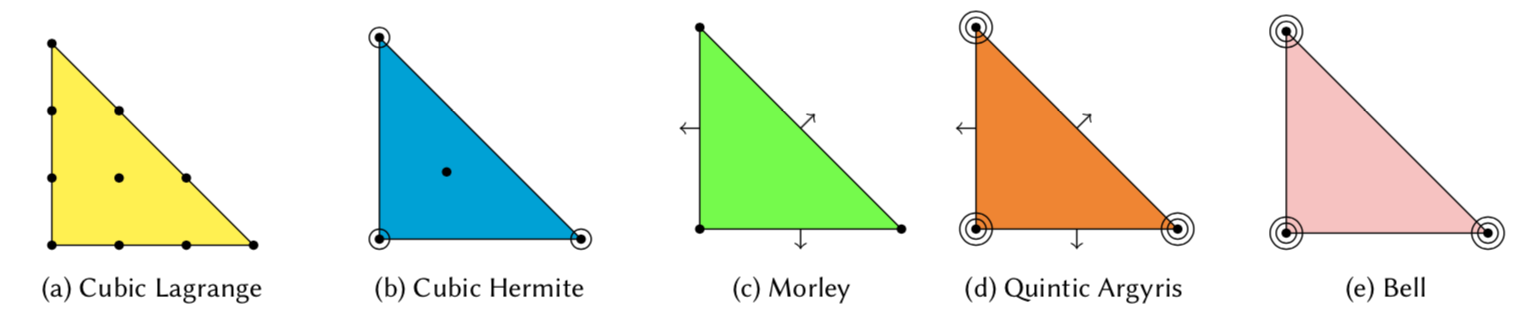
\includegraphics[width=0.8\textwidth]{elements}
  \end{center}
\end{frame}

\begin{frame}
  \frametitle{Pictures}
  \begin{center}
    \only<1>{
      Eigenmodes of the clamped plate problem
      \begin{equation*}
        \Delta^2 u = f
      \end{equation*}

      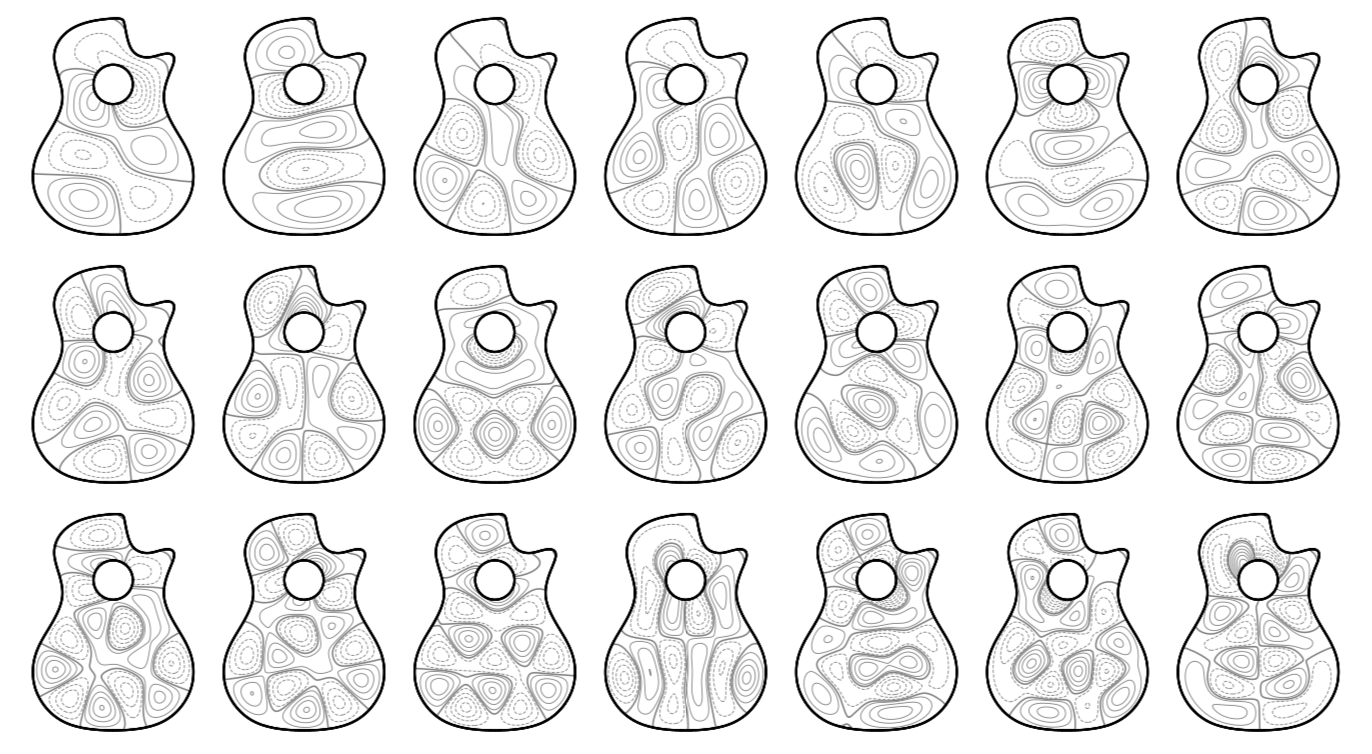
\includegraphics[width=\textwidth]{eigenmodes}
    }
    \only<2>{
      Sea surface salinity at outflow of the Columbia river (with
      \url{thetisproject.org}).
      
      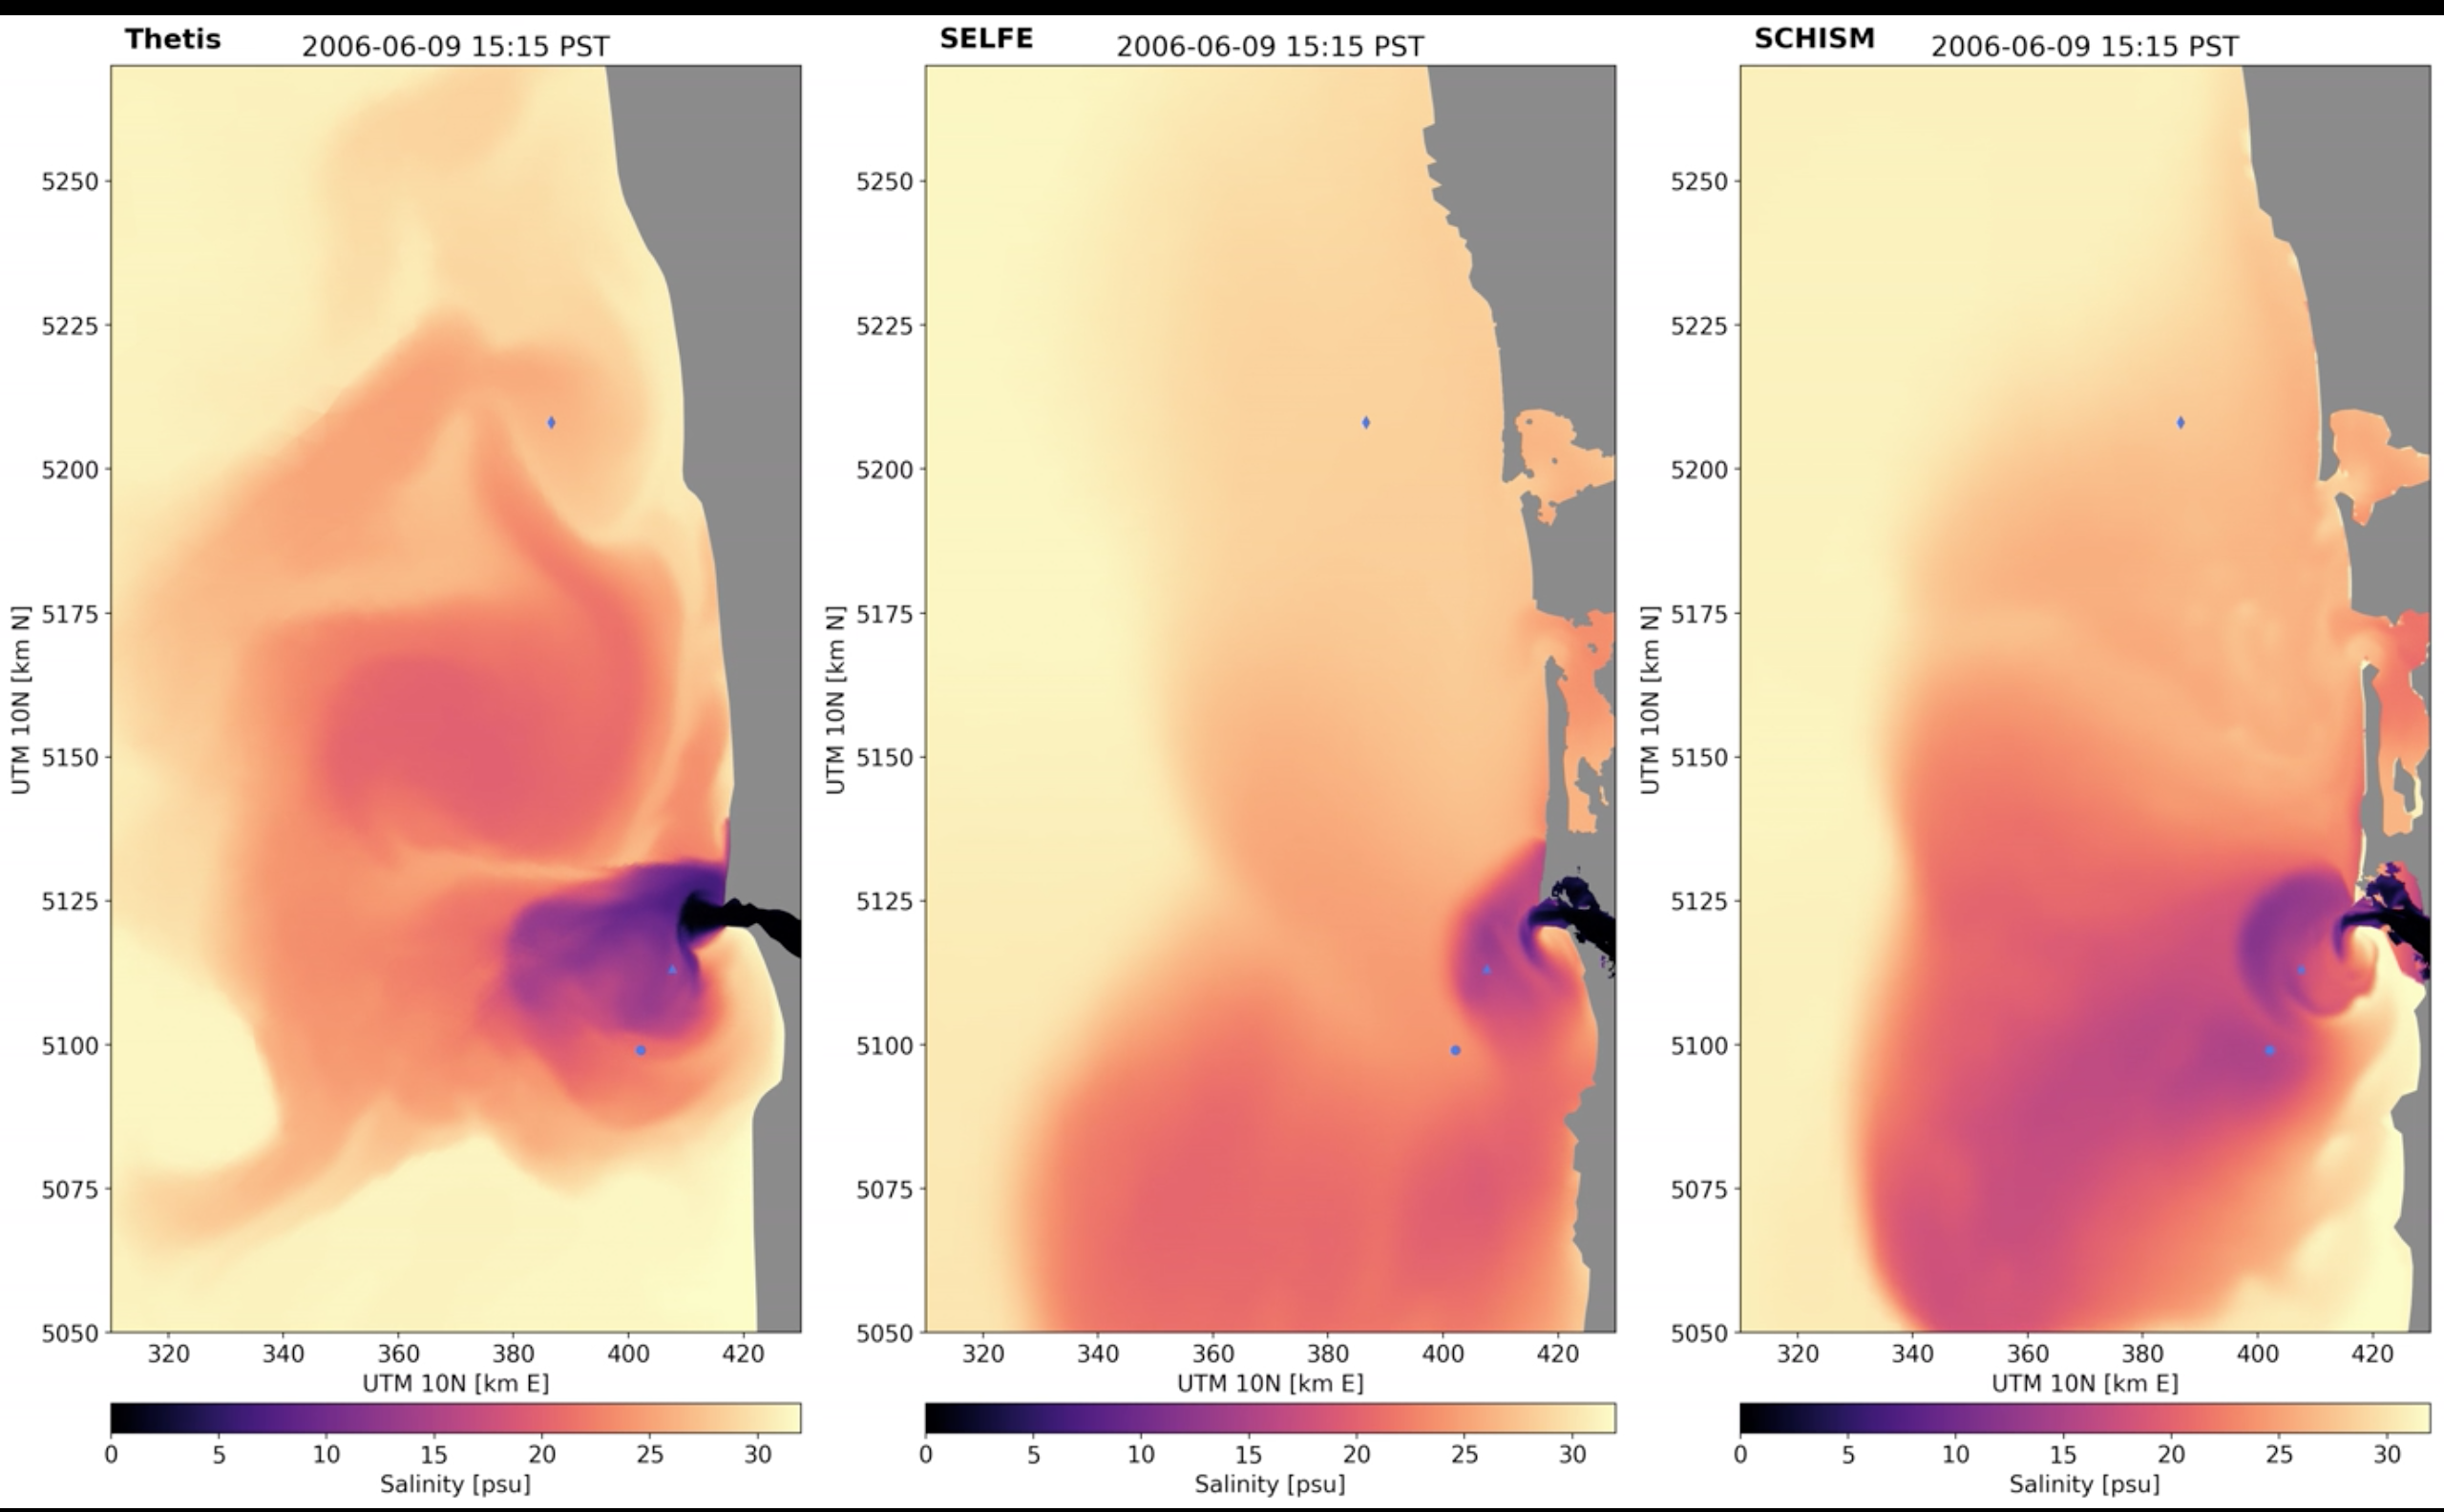
\includegraphics[width=\textwidth]{thetis-snapshot}
    }
  \end{center}
\end{frame}

\begin{frame}
  \frametitle{Multilevel preconditioning}
  \begin{itemize}
  \item Scalable linear solvers for most PDEs require multilevel
    preconditioning
  \item Takes advantage of hierarchy of scales
  \item Challenge is to create solvers that are \emph{robust} to the parameters
  \end{itemize}

  \begin{block}{Incompressible Navier--Stokes}
    \begin{align*}
      - \nu \nabla^2 u + (u \cdot \nabla) u + \nabla p &= f\\
      \nabla \cdot u &= 0 
    \end{align*}
    Challenging to solve in $\lim_{\nu \to 0}$ (high Reynolds number).
  \end{block}
\end{frame}

\begin{frame}
  \frametitle{Geometric multigrid scheme}
  \begin{itemize}
  \item Reynolds-robust multigrid scheme for 3D Navier--Stokes
    {\small \arxivlink{1810.03315}{math.NA}}
    \begin{columns}
      \begin{column}{0.6\pagewidth}
        {\footnotesize
          \begin{table}[htbp]
            \centering
            \begin{tabular}{c|ccccc}
              \toprule
              \# dofs & \multicolumn{5}{c}{Reynolds number} \\
                      & 10 & 100 & 1000 & 2500 & 5000 \\
              \midrule
              $2.1 \times 10^6$ & 7.50 & 7.33 & 7.50 & 7.00 & 6.50 \\
              $1.7 \times 10^7$ & 8.50 & 7.00 & 7.50 & 6.50 & 5.50 \\
              $1.3 \times 10^8$ & 7.00 & 7.00 & 6.50 & 5.00 & 6.50 \\
              $1.1 \times 10^9$ & 7.00 & 7.33 & 5.50 & 4.00 & 9.00 \\
              \bottomrule
            \end{tabular}
            \caption{Krylov iterations per Newton step}
          \end{table}
        }
      \end{column}
      \begin{column}{0.4\pagewidth}
        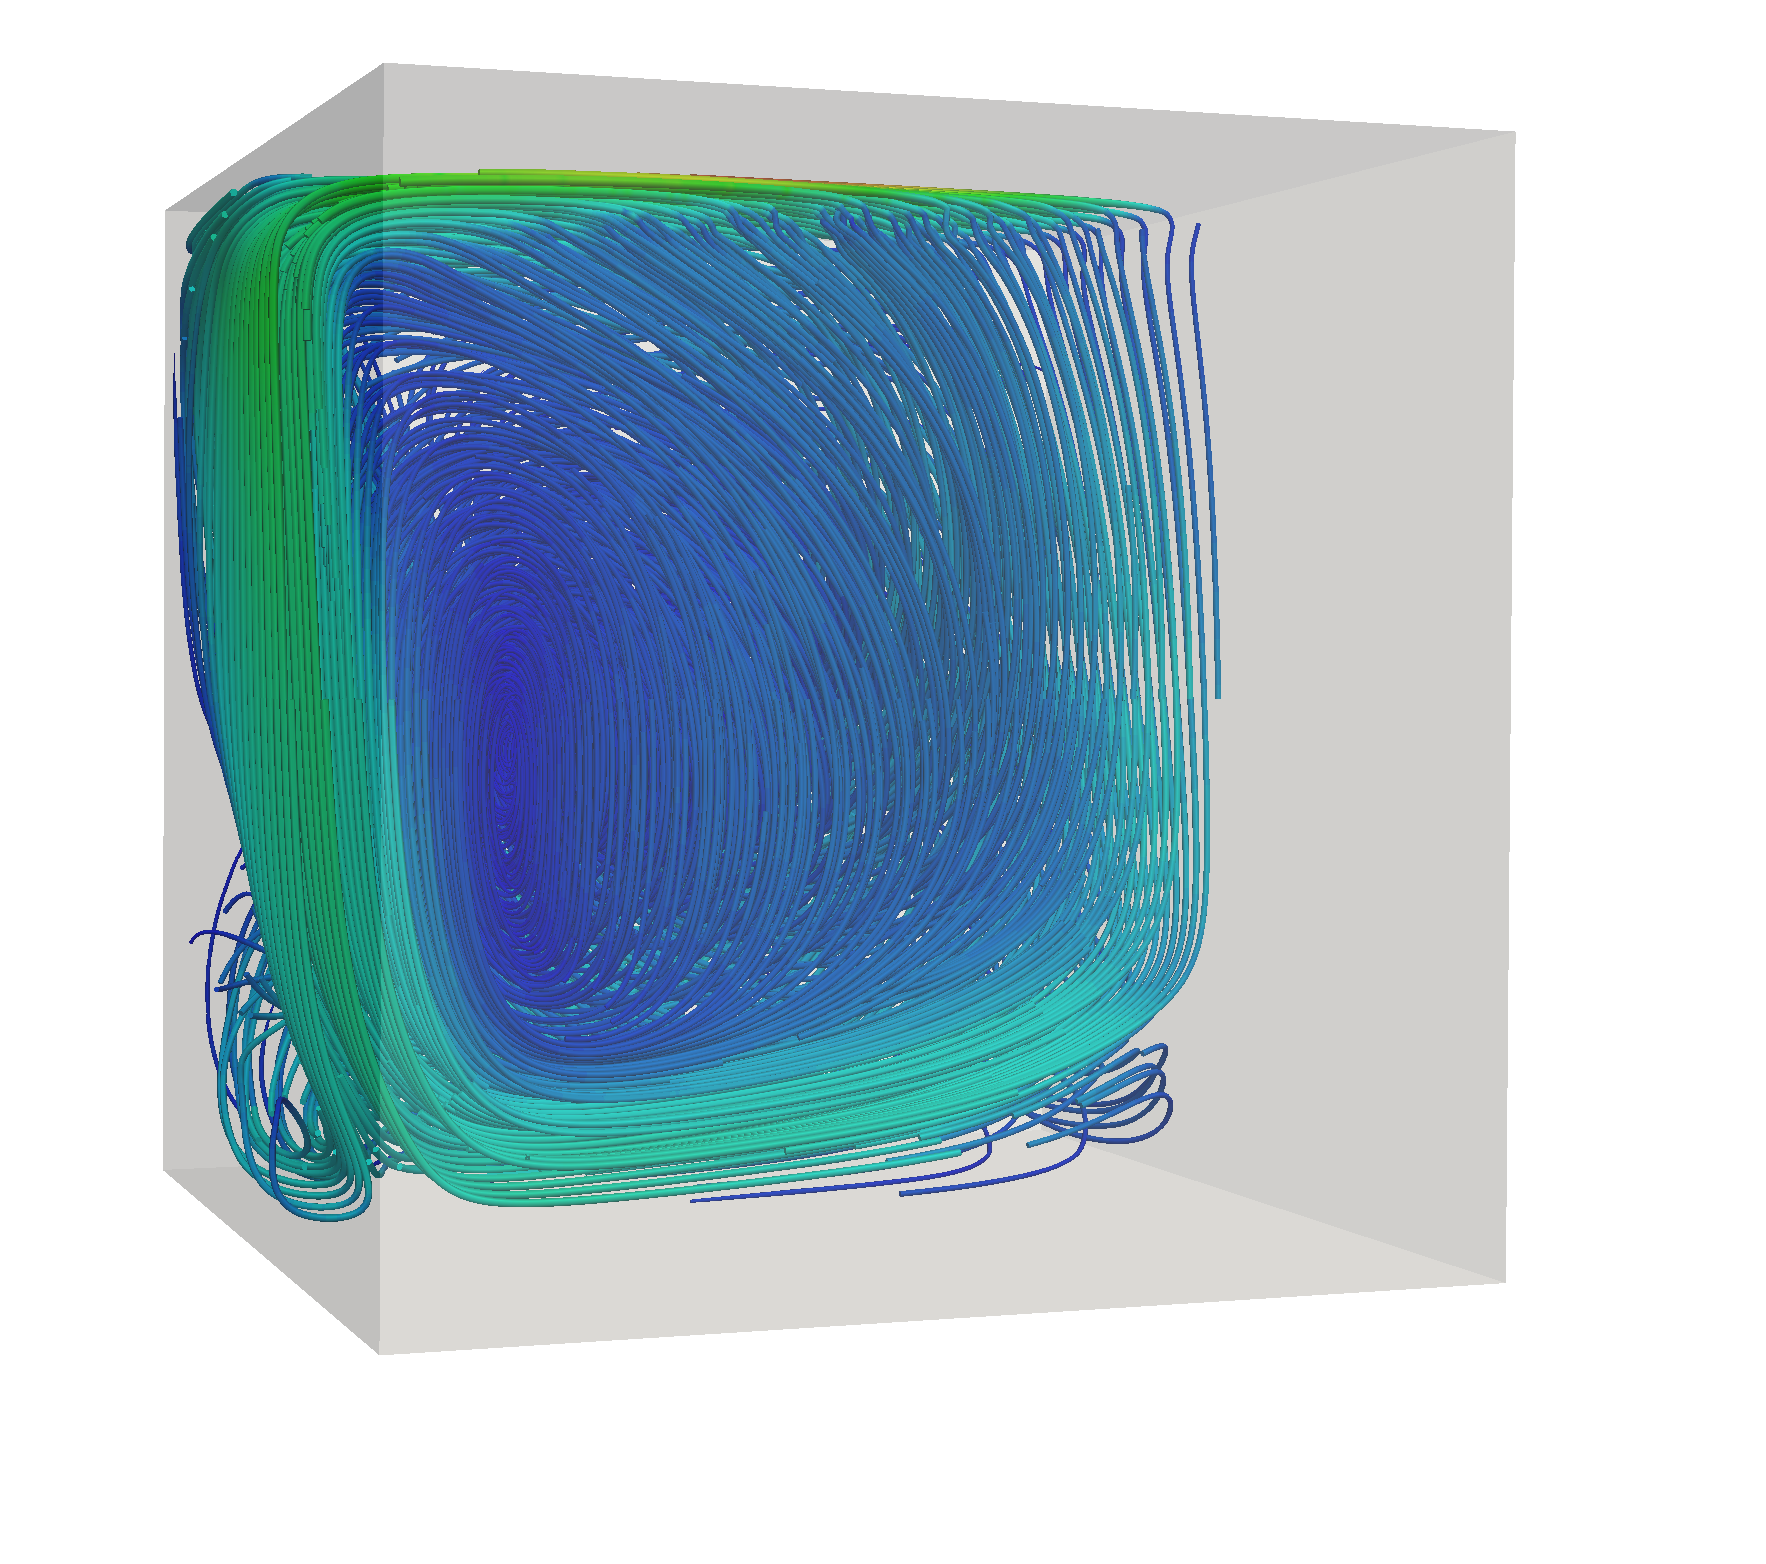
\includegraphics[width=1\textwidth]{LDC-streamlines}
      \end{column}
    \end{columns}
  \item Now looking at
    \begin{itemize}
    \item Transient (easier)
    \item Exactly divergence-free discretisations (harder)
    \item Nonlinear rheologies (probably harder)
    \item Same ideas apply to nearly incompressible elasticty
    \end{itemize}
  \end{itemize}
\end{frame}

\begin{frame}
  \frametitle{Summary}
  \begin{itemize}
  \item Finite elements can be fun!
  \item Code all available \url{www.firedrakeproject.org}
  \end{itemize}

  \begin{center}
    \LARGE

    Demo, movies, while

    Questions?
  \end{center}
\end{frame}
\end{document}
